\chapter{固有時、時間の遅れ、長さの収縮}

我々はしばしば光速が$c=1$である単位系を選ぶ。この単位系では、年で表した時間と光年で表した距離を直接比較でき、式はずっと読みやすくなる。$c$が物理的に重要になる場合は常に、それを復元する。次元解析だけでそれを特定するのに十分である。

\section{ガリレイ的時空格子}

静止系と、$x$軸に沿って速度$v$で運動する列車との間のアインシュタイン以前の関係から始めよう：
\begin{align}
x' &= x-vt, & t'&=t.
\label{eq:l4-galilean}
\end{align}
第2の式にはニュートンの絶対時間の仮定が含まれている。空間原点が互いに相対的に動いていても、すべての観測者は同じ同時刻のスライスを用いる。

プライムなしの観測者が線路のそばに立ち、プライム付きの観測者が列車に乗っているとしよう。列車の原点は$x'=0$であるから、プライムなし座標におけるその世界線は
\begin{equation}
x=vt.
\end{equation}
である。この傾いた直線が$t'$軸である。対照的に、$t'=t$は、$t'$が一定のすべての直線が$t$が一定の直線と同じ水平線であることを述べている。

\begin{figure}[H]
\centering
\includegraphics[width=0.72\textwidth]{lecture_04_figure_02.png}
\caption{ガリレイ変換と初期の$t$-$x$格子。運動する原点は$x=vt$を描くが、二つの系は共通の等時間線を保つ。}
\lectureframe{00:03:06}
\end{figure}

式~\eqref{eq:l4-galilean}をプライムなし座標について解くと
\begin{align}
x&=x'+vt'=x'+vt, & t&=t'.
\end{align}
が得られる。逆変換は$v$を$-v$に置き換えた同じ形をしている。列車が駅に対して前進するなら、駅は列車に対して後退する。この相互性は特殊相対性理論でも生き残るが、絶対時間は生き残らない。

\section{ローレンツ補正}

ガリレイ変換は、すべての慣性系で光速を同じにすることはできない。修正された関係は、まず$c=1$単位で、
\begin{align}
x'&=\frac{x-vt}{\sqrt{1-v^2}}, &
t'&=\frac{t-vx}{\sqrt{1-v^2}}.
\label{eq:l4-lorentz-natural}
\end{align}
である。通常の単位を復元すると
\begin{align}
x'&=\frac{x-vt}{\sqrt{1-v^2/c^2}}, &
t'&=\frac{t-vx/c^2}{\sqrt{1-v^2/c^2}}.
\label{eq:l4-lorentz-c}
\end{align}
となる。

\begin{figure}[H]
\centering
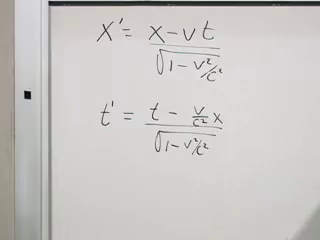
\includegraphics[width=0.74\textwidth]{lecture_04_figure_05.png}
\caption{$c$の因子を復元したローレンツ変換。}
\lectureframe{00:09:10}
\end{figure}

$v\ll c$では、ニュートン力学が用いられる状況において$v^2/c^2$と$vx/c^2$はどちらも微小である。そのとき式~\eqref{eq:l4-lorentz-c}はガリレイ的結果に帰着する。相対性理論はニュートン的運動学を捨て去るのではなく、その有効範囲を特定するのである。

$v=c$では、分母が消える。一つの慣性系が別の慣性系に対して光速で運動することはできない。その極限より十分下では補正は小さいが、その近くでは$x$と$t$の混合が避けられなくなる。

運動は$x$に沿って選ばれたので、横方向の座標は変化しない：
\begin{equation}
y'=y,\qquad z'=z.
\end{equation}
その理由を見る一つの方法は、列車とプラットフォームに同一の横方向の物差しを置くことである。二つの系の中間を運動する観測者は、棒が等しく反対向きの速度で近づいてくるのを見る。この設定には、一方の横方向の棒を他方より短くしうる特徴が何もない。

\section{光円錐に沿ったローレンツ変換}

式~\eqref{eq:l4-lorentz-natural}を読む幾何学的な方法がある。その二つの式を加える：
\begin{align}
t'+x'
&=\frac{(t-vx)+(x-vt)}{\sqrt{1-v^2}}\\
&=(t+x)\frac{1-v}{\sqrt{1-v^2}}\\
&=(t+x)\sqrt{\frac{1-v}{1+v}}.
\label{eq:l4-null-plus}
\end{align}
補完的な順序で引く：
\begin{align}
t'-x'
&=\frac{(t-vx)-(x-vt)}{\sqrt{1-v^2}}\\
&=(t-x)\frac{1+v}{\sqrt{1-v^2}}\\
&=(t-x)\sqrt{\frac{1+v}{1-v}}.
\label{eq:l4-null-minus}
\end{align}

\begin{figure}[H]
\centering
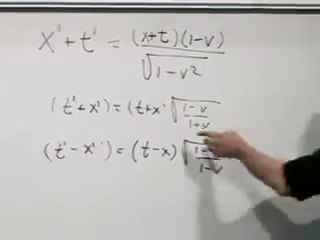
\includegraphics[width=0.75\textwidth]{lecture_04_figure_06.png}
\caption{ローレンツ変換をヌル結合$t+x$と$t-x$で書き直したもの。それらのスケール因子は互いに逆数である。}
\lectureframe{00:18:45}
\end{figure}

結合$t+x$と$t-x$は、二つの$45^\circ$光的方向に沿った座標である。ブーストはこれらの方向の一方を縮め、他方を逆因子で伸ばす。どちらかを$45^\circ$から回転させて離すことはない。したがって光線は光線のままであり、これが光速不変の時空的な描像である。

\begin{classroomqa}
\audiencequestion{中間の観測者は対称な実験を見るが、それによって列車とプラットフォームの観測者に対する結果がどのように確立されるのか。\lecturetimestamp{00:20:48}}
\lecturerresponse{もう一つの事実が用いられている：事象の一致は不変である。棒の端が出会うなら、その出会いは一つの時空事象である。すべての慣性観測者はそれに異なる座標を割り当ててよいが、一つの一致を二つの異なる位置に分けることはできない。対応する端点が出会う場所で発せられる閃光は、それらの事象を操作的に検出可能にする。中間系の対称性と二つの端点一致の不変性が、横方向の長さが一致することを確立する。}
\end{classroomqa}

\begin{classroomqa}
\audiencequestion{中間の慣性系を代表する自転車乗りは、棒の中点に物理的に位置していなければならないのか。\lecturetimestamp{00:22:25}}
\lecturerresponse{いいえ。基準系とは観測者と時計からなる一つの網全体であり、ある一点にある一つの目ではない。自転車乗りは端点の発光を後で受け取り、それらがどこから発せられたかを推論してもよい。重要なのは各発光事象の時空上の位置であり、光が最終的にどこで受信されるかではない。}
\end{classroomqa}

逐次的な速度の合成も同じ変換のもう一つの帰結であるが、それは意図的に次の講義に残される。現在の課題は、運動する時計が測る不変量を特定することである。

\section{不変間隔}

通常のデカルト軸の回転では、量$x^2+y^2$は不変である。ローレンツ変換は異なる二次形式を保存する。式~\eqref{eq:l4-lorentz-natural}より、
\begin{align}
t'^2-x'^2
&=\frac{(t-vx)^2-(x-vt)^2}{1-v^2}\\
&=\frac{t^2-2vtx+v^2x^2-x^2+2vtx-v^2t^2}{1-v^2}\\
&=t^2-x^2.
\label{eq:l4-interval}
\end{align}
混合項は相殺され、残った分子は共通因子$1-v^2$を含む。

\begin{figure}[H]
\centering
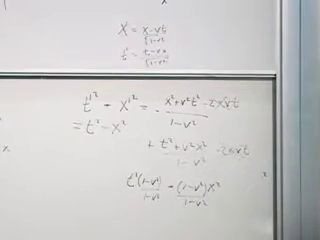
\includegraphics[width=0.76\textwidth]{lecture_04_figure_07.png}
\caption{$t'^2-x'^2=t^2-x^2$の板書による導出。}
\lectureframe{00:33:15}
\end{figure}

3つの空間次元がある場合、不変量は
\begin{equation}
t'^2-x'^2-y'^2-z'^2=t^2-x^2-y^2-z^2
\end{equation}
であり、$c=1$単位で表される。より一般には、2つの事象に対して座標差を用いる：
\begin{equation}
\Delta s^2
=c^2\Delta t^2-\Delta x^2-\Delta y^2-\Delta z^2.
\label{eq:l4-spacetime-interval}
\end{equation}
すべての慣性観測者は、その時間項と空間項を別々には一致させないが、この数については一致する。

\section{固有時と運動する時計}

光信号を交換して同期された時計を持つ静止観測者の格子を想像せよ。それらの読みは座標時$t$を定義する。次に、一つの腕時計をその格子の中を運んでいこう。その時計自身の読みは世界線に沿って時計に従う。その読みが固有時である。

時間的に分離された2つの事象に対して、
\begin{equation}
c^2\Delta\tau^2
=c^2\Delta t^2-\Delta x^2-\Delta y^2-\Delta z^2.
\label{eq:l4-proper-time}
\end{equation}
と定義する。$c=1$である1つの空間次元では、これは単に
\begin{equation}
\Delta\tau=\sqrt{\Delta t^2-\Delta x^2}.
\end{equation}
となる。平方根は通常の距離の公式と類似しているが、マイナス符号が幾何学を変える。

3つの場合がある：
\begin{align}
\Delta t^2-\Delta x^2 &>0 &&\text{timelike},\\
\Delta t^2-\Delta x^2 &=0 &&\text{lightlike},\\
\Delta t^2-\Delta x^2 &<0 &&\text{spacelike}.
\end{align}
光円錐の内部では固有時は実である。光円錐上では、$x=\pm t$であり、事象が一致する必要はないにもかかわらず、固有時はゼロである。光線はまさにそのような事象を結ぶことができる。光円錐の外部では分離は空間的であり、虚数の時計時間よりも実の固有距離$\sqrt{\Delta x^2-\Delta t^2}$で記述する方がよい。

\begin{figure}[H]
\centering
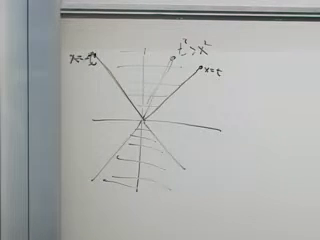
\includegraphics[width=0.73\textwidth]{lecture_04_figure_08.png}

\vspace{0.8em}

\begin{tikzpicture}[x=1.0cm,y=1.0cm]
\draw[->] (-3.3,0) -- (3.3,0) node[right] {$x$};
\draw[->] (0,-0.4) -- (0,4.0) node[above] {$t$};
\draw[thick] (0,0) -- (3.0,3.0) node[above right] {$x=t$};
\draw[thick] (0,0) -- (-3.0,3.0) node[above left] {$x=-t$};
\node at (0,2.0) {timelike};
\node at (2.25,1.05) {spacelike};
\node at (-2.25,1.05) {spacelike};
\end{tikzpicture}
\caption{板書の光円錐と、時間的、光的、空間的分離の明確な分類。}
\lectureframe{00:38:40}
\end{figure}

なぜ式~\eqref{eq:l4-proper-time}は時計の読みに等しいのか。静止している時計では$\Delta x=0$なので、$\Delta\tau=\Delta t$である。一様に運動する時計では、その時計が静止しているプライム付きの系を選ぶ。そこでは$\Delta x'=0$であり、不変性により
\begin{equation}
\Delta\tau
=\sqrt{\Delta t'^2-\Delta x'^2}
=\Delta t'.
\end{equation}
したがって、運動する時計は固有時を刻む。

\begin{classroomqa}
\audiencequestion{``事象間の間隔''と``時計の読み''は、同じものの2つの名前として使われているのか。
\lecturetimestamp{00:44:49}}
\lecturerresponse{理想的な時計が一方の事象から他方の事象へ慣性運動で進むとき、それらは一致する。不変間隔は幾何学的量であり、共動時計の端点の読みの差はその物理的測定である。静止した座標時計は一般に異なる座標時間間隔を記録する。}
\end{classroomqa}

\section{時間の遅れと同時性}

運動する系の原点を考えよ。その世界線は
\begin{equation}
x'=0,\qquad x=vt.
\end{equation}
に従う。同じ傾いた直線は、運動する時計の経路でもあり、$t'$軸でもある。

\begin{figure}[H]
\centering
\includegraphics[width=0.72\textwidth]{lecture_04_figure_03.png}
\caption{運動する原点：$x=vt$、$x'=0$、および$t'$軸は、同じ世界線の3つの記述である。}
\lectureframe{00:48:18}
\end{figure}

共通の原点とその世界線上の後の点との間に不変間隔を適用する：
\begin{align}
t'^2-x'^2&=t^2-x^2,\\
t'^2&=t^2-v^2t^2,\\
t'&=t\sqrt{1-v^2}.
\label{eq:l4-time-dilation-natural}
\end{align}
$c$を復元すると、
\begin{equation}
\Delta\tau=\Delta t\sqrt{1-\frac{v^2}{c^2}}
=\frac{\Delta t}{\gamma},
\qquad
\gamma=\frac{1}{\sqrt{1-v^2/c^2}}.
\label{eq:l4-time-dilation}
\end{equation}

\begin{figure}[H]
\centering
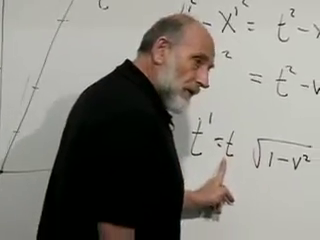
\includegraphics[width=0.73\textwidth]{lecture_04_figure_09.png}
\caption{板書の時間の遅れの結果：運動する時計は、$c=1$である単位で$t'=t\sqrt{1-v^2}$を蓄積する。}
\lectureframe{00:50:45}
\end{figure}

静止観測者は、運動する時計が遅れると言う。相互性により、運動する観測者も静止した時計について同じことを言わなければならない。2つの記述は異なる遠方の事象の対を比較するので、矛盾はない。

実際、式~\eqref{eq:l4-lorentz-natural}において$t'$が一定であることは
\begin{equation}
t-vx=\text{constant}.
\label{eq:l4-simultaneity}
\end{equation}
を満たす。運動する観測者の同時線は、水平線$t=\text{constant}$に対して傾いている。各観測者は、異なる遠方の時計の読みの集合を同時であると呼ぶ。その違いを可視化しておけば、時計の相互的な遅れは整合している。

\begin{figure}[H]
\centering
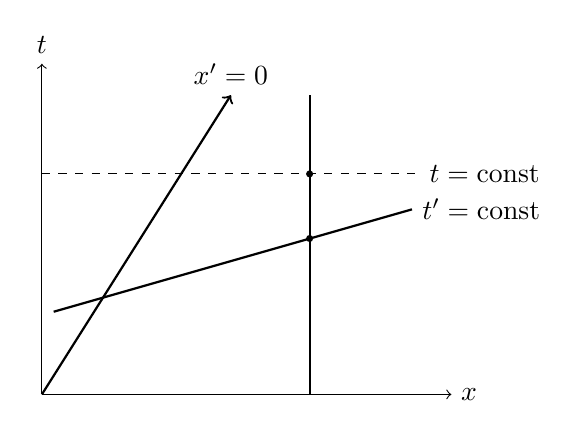
\begin{tikzpicture}[x=1cm,y=1cm]
\draw[->] (0,0) -- (0,4.2) node[above] {$t$};
\draw[->] (0,0) -- (5.2,0) node[right] {$x$};
\draw[thick,->] (0,0) -- (2.4,3.8) node[above] {$x'=0$};
\draw[dashed] (0,2.8) -- (4.8,2.8)
  node[right] {$t=\mathrm{const}$};
\draw[thick] (0.15,1.05) -- (4.7,2.35)
  node[right] {$t'=\mathrm{const}$};
\draw[thick] (3.4,0) -- (3.4,3.8);
\fill (3.4,2.8) circle (0.045);
\fill (3.4,1.98) circle (0.045);
\end{tikzpicture}
\caption{相互的な時間の遅れは、異なる同時面における時計の読みを比較する。}
\end{figure}

\section{双子の経路}

二人の双子が同じ事象から出発する。一方は$x=0$にとどまる。他方は速さ$v$で外へ向かって進み、向きを反転して同じ速さで戻る。再会したとき、彼らは時計として働きうるあらゆる物理過程を比較する。腕時計、心拍、代謝、あるいは老化そのものである。

旅行の各半分が、家にいる系で座標時間$T$かかるとする。家にいる双子の固有時間は
\begin{equation}
\tau_{\mathrm{home}}=2T.
\end{equation}
である。折り返しの事象の座標は$(vT,T)$である。したがって行きの脚は
\begin{align}
\tau_{\mathrm{leg}}
&=\sqrt{T^2-v^2T^2}
=T\sqrt{1-v^2}.
\end{align}
に寄与する。帰りの脚も同じ量に寄与するので、
\begin{equation}
\tau_{\mathrm{travel}}=2T\sqrt{1-v^2}<2T.
\label{eq:l4-twin}
\end{equation}
となる。

\begin{figure}[H]
\centering
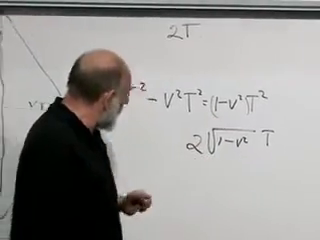
\includegraphics[width=0.73\textwidth]{lecture_04_figure_10.png}

\vspace{0.8em}

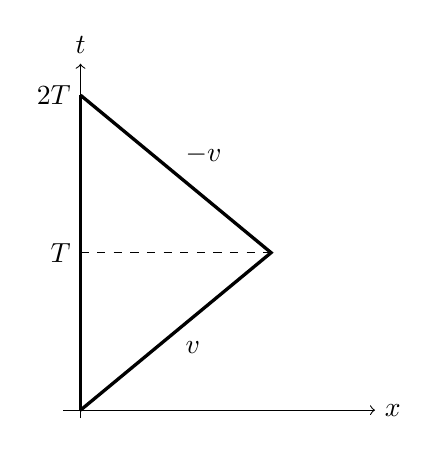
\begin{tikzpicture}[x=1.1cm,y=1cm]
\draw[->] (-0.2,0) -- (3.4,0) node[right] {$x$};
\draw[->] (0,-0.1) -- (0,4.4) node[above] {$t$};
\draw[very thick] (0,0) -- (0,4);
\draw[very thick] (0,0) -- (2.2,2) -- (0,4);
\draw[dashed] (0,2) -- (2.2,2);
\node[left] at (0,2) {$T$};
\node[left] at (0,4) {$2T$};
\node[below right] at (1.1,1.0) {$v$};
\node[above right] at (1.1,3.0) {$-v$};
\end{tikzpicture}
\caption{家にいる世界線と二つの旅行の脚。それらの固有時間が異なるのは、それらが時空を通る異なる経路だからである。}
\lectureframe{00:59:35}
\end{figure}

年齢が等しくないことに矛盾はない。旅行の経路は折り返しを含み、まっすぐな家の経路とは単一の慣性系の対称性によって関係づけられない。通常のユークリッド幾何学でも、二点間のまっすぐな経路と折れ曲がった経路は異なる長さをもつ。ミンコフスキー幾何学では、どちらの経路がより大きな間隔をもつかは逆になるが、比較は依然として幾何学的である。

\section{加速度と理想時計}

\begin{classroomqa}
\audiencequestion{折り返しでは物理が異なり、旅行者は加速する。それは時計の計算を無効にするのだろうか。
\lecturetimestamp{01:02:19}}
\lecturerresponse{加速度は実在し、非対称性を特定するのに役立つ。それを議論で消し去るべきではない。鋭い角は単に理想化された作図であり、有限の折り返しに丸めてもよい。さらなる物理的仮定は、十分に小さく、よく作られた時計は適度な加速度に敏感でなく、固有時間を記録し続けるというものである。大きな時計や壊れやすい時計は変形したり壊れたりするかもしれないが、それは時空間隔の欠陥ではなく、機構の欠陥である。}
\end{classroomqa}

この理想時計の仮定は、ローレンツ変換だけから導かれるものではない。それは実際の時計機構の振る舞いを通じて検証される。原子は、何百マイルもの大きさの時計よりもはるかに良い近似である。なぜなら、コンパクトな機構は加速度や重力のもとで歪みにくいからである。一般相対性理論の名を挙げても、この物理的問題は解消しない。選んだ機構がその環境にどう応答するかを、依然として知らなければならないのである。

\begin{classroomqa}
\audiencequestion{加速された軌道を、慣性解析が有効なままである短い区間に還元できるだろうか。\lecturetimestamp{01:09:08}}
\lecturerresponse{できる。曲線を短くほぼまっすぐな線分に分割し、各区間で固有時間を計算し、その結果を足し合わせる。これは、通常の曲線の長さを多くの小さな線分から求めることの時空版である。連続極限では、
\[
\tau=\int \sqrt{1-\frac{v(t)^2}{c^2}}\,dt,
\]
となる。これは、慣性座標系で記述された平坦な時空内の運動に対するものである。}
\end{classroomqa}

\section{双子が見るもの}

最終的な時計の読みは、光パルスを送ることによって操作的に定められる。両方の世界線上に固有時間の1秒間隔を印し、各双子が各印でパルスを放出するとする。行きの脚では、相手の双子から受け取るパルスは間隔が広がる。帰りの脚では、それらは詰まって到着する。これは時空図の上で直接表された相対論的ドップラー効果である。

\begin{figure}[H]
\centering
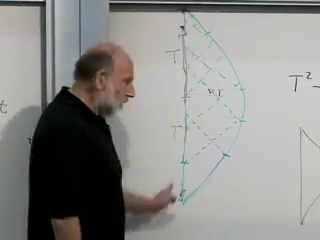
\includegraphics[width=0.73\textwidth]{lecture_04_figure_11.png}
\caption{家の世界線と旅行の世界線の間で交換される光信号。行きの脚でのまばらな到着と帰りの脚での圧縮された到着が、放出されたすべてのパルスを説明する。}
\lectureframe{01:12:55}
\end{figure}

この話のどの系も消え去らない。各観測者は最終的に相手が放出したすべてのパルスを受け取るが、その受信率は相対運動に依存する。行きの赤方偏移と帰りの青方偏移は、二つの経路にとって等しい持続時間の効果ではない。したがって、受け取ったすべてのパルスを数えることは固有時間の比較と一致する。

\begin{classroomqa}
\audiencequestion{戻ってくる旅行者が青方偏移した光を受け取るなら、旅行者は光源が放出したよりも多くのエネルギーを集められるだろうか。
\lecturetimestamp{01:13:50}}
\lecturerresponse{その問いには、エネルギーの相対論的定義と系依存性が必要であり、それらはまだ展開されていない。もっともではあるが、座標とパルス数だけでは、特に加速された観測者について、エネルギーの収支を決着させるのに十分ではない。したがって、答えは推測するのではなく後回しにすべきである。}
\end{classroomqa}

\section{閉じた空間方向}

\begin{classroomqa}
\audiencequestion{空間方向の一つがコンパクトであるとしよう。双子の一方はその方向に沿って一様に運動し、出発点に戻り、加速度をまったく避けることができるだろうか。そのとき、何が双子を区別するのか。\lecturetimestamp{01:15:14}}
\lecturerresponse{空間は、より大きな空間の中に曲げ込まれた一枚の紙としてではなく、内在的に円筒として想像されるべきである。動径方向の加速度は必要ない。それでも、戻ってくる観測者は、同じ場所が再び現れるという大域的な事実に遭遇する。これは非対称性を示しているが、完全な答えには、空間的同一視を伴う特殊相対性理論の注意深い取り扱いが必要である。この問いは、その場しのぎで答えるのではなく、ここでは未解決のままにしておく。}
\end{classroomqa}

\begin{figure}[H]
\centering
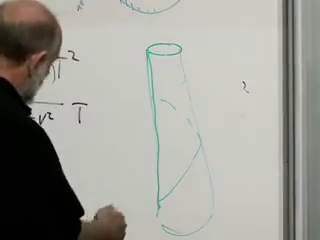
\includegraphics[width=0.72\textwidth]{lecture_04_figure_04.png}

\vspace{0.8em}

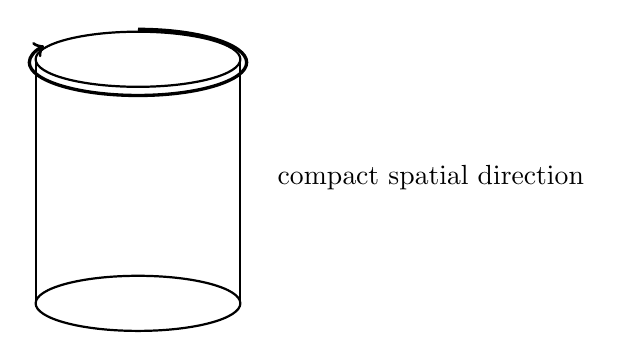
\begin{tikzpicture}[x=1cm,y=1cm]
\draw[thick] (0,0) ellipse (1.3 and 0.35);
\draw[thick] (-1.3,0) -- (-1.3,-3.1);
\draw[thick] (1.3,0) -- (1.3,-3.1);
\draw[thick] (0,-3.1) ellipse (1.3 and 0.35);
\draw[->,very thick] (0.0,0.38) arc (90:-210:1.38 and 0.42);
\node[right] at (1.65,-1.5) {compact spatial direction};
\end{tikzpicture}
\caption{黒板に描かれたコンパクト空間の問い。清潔な内在的円筒とともに。これは、余分な動径次元に埋め込まれた円筒の周りを運動することではなく、大域的同一視に関する問いである。}
\lectureframe{01:17:56}
\end{figure}

\section{長さは同時刻面で測られる}

特殊相対性理論の問題では、まず時空図を描く。プライムなしの系で静止しているメートル棒を取り、その端点を$x=0$と$x=1$に置く。時間が経つにつれて、二つの端点は垂直な世界線を描く。棒はそれらの間にリボンを掃き出す。

運動している観測者は、運動している時間$t'$の一つの値で両方の端点を測らなければならない。式~\eqref{eq:l4-simultaneity}から、原点を通り$t'=0$である面は、$c=1$単位で
\begin{equation}
t=vx
\end{equation}
を満たす。それは右の端点$x=1$と$t=v$で交わる。

\begin{figure}[H]
\centering
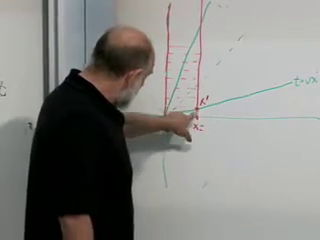
\includegraphics[width=0.73\textwidth]{lecture_04_figure_12.png}

\vspace{0.8em}

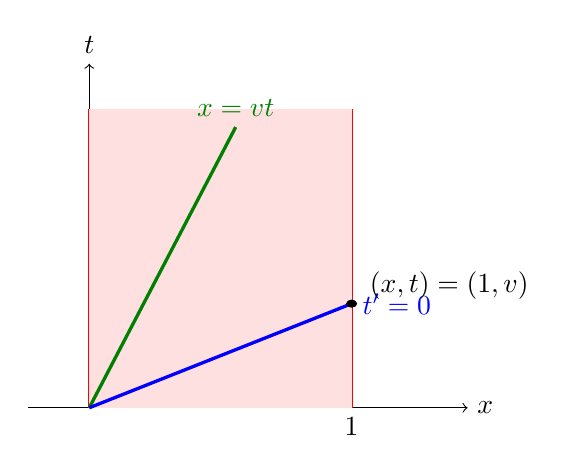
\begin{tikzpicture}[x=1.55cm,y=1.15cm]
\draw[->] (-0.5,0) -- (3.1,0) node[right] {$x$};
\draw[->] (0,0) -- (0,3.8) node[above] {$t$};
\draw[very thick,red] (0,0) -- (0,3.3);
\draw[very thick,red] (2.15,0) -- (2.15,3.3);
\fill[red!12] (0,0) rectangle (2.15,3.3);
\draw[very thick,green!50!black] (0,0) -- (1.2,3.1)
  node[above] {$x=vt$};
\draw[very thick,blue] (0,0) -- (2.15,1.15)
  node[right] {$t'=0$};
\fill (2.15,1.15) circle (0.045);
\node[right] at (2.22,1.35) {$(x,t)=(1,v)$};
\node[below] at (2.15,0) {$1$};
\end{tikzpicture}
\caption{静止している棒は時空のリボンを掃き出す。運動している観測者にとっての長さは、一つの$t'=\mathrm{const}$面におけるその端点間の隔たりである。}
\lectureframe{01:24:20}
\end{figure}

選ばれた端点の隔たりは空間的であるから、不変量の正の空間的形式を用いる：
\begin{equation}
x'^2-t'^2=x^2-t^2.
\end{equation}
選ばれた端点では、$t'=0$、$x=1$、そして$t=v$である。したがって
\begin{align}
x'^2&=1-v^2,\\
x'&=\sqrt{1-v^2}.
\end{align}
よって、静止長$L$は、運動している系で
\begin{equation}
L'=L\sqrt{1-v^2/c^2}=\frac{L}{\gamma}.
\label{eq:l4-length-contraction}
\end{equation}
と測られる。

\begin{figure}[H]
\centering
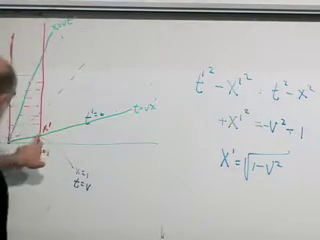
\includegraphics[width=0.76\textwidth]{lecture_04_figure_13.png}
\caption{完成した長さの収縮の作図と、単位静止長に対する黒板の結果$x'=\sqrt{1-v^2}$。}
\lectureframe{01:28:10}
\end{figure}

逆の主張もまた成り立つ：プラットフォームの観測者は、列車の縦方向のメートル棒により短い長さを割り当てる。ここでもまた、二人の観測者は異なる同時的な端点事象を選ぶので、相互性は矛盾ではない。

\section{最後の質問}

\begin{classroomqa}
\audiencequestion{光以外に光速で伝播するものはあるか。特に、重力はどうか。\lecturetimestamp{01:29:29}}
\lecturerresponse{一般相対性理論は、$c$で伝播する重力波を予言する。この講義の時点では、証拠は連星パルサーなどの系から間接的に得られており、重力波はまだ直接検出されていなかった。\editorialnote{実験状況はこの2006年の講義の後に変わった。LIGOは2015年にGW150914を直接検出し、2017年におけるGW170817とその電磁対応物の同時観測は、重力と光の伝播速度が$10^{15}$分の数以内で一致することを示した。\url{https://ligo.org/detections/gw150914/}と
\url{https://doi.org/10.1103/PhysRevLett.119.251302}を参照。}}
\end{classroomqa}

\begin{classroomqa}
\audiencequestion{宇宙飛行士は、何光年もの距離を、その距離を光年で表した値よりも短い固有時間で横切ることができるだろうか。それは光より速く動くことを意味するだろうか。\lecturetimestamp{01:30:38}}
\lecturerresponse{宇宙飛行士の固有時間は
$\sqrt{\Delta t^2-\Delta x^2}$であり、これは座標時間
$\Delta t$より小さい。宇宙飛行士の慣性系では、星々の間の距離はローレンツ収縮している。星々は速度$-v$で動いており、光より速くはない。横切るべき収縮した距離が単に小さいだけである。}
\end{classroomqa}

宇宙飛行士が静止から始めて加速する場合、記述は一連の瞬間的慣性系の間で変化する。星々に割り当てられる距離は、その移行の間に変化しうる。一つの固定したローレンツ変換を加速された全履歴に適用することはできないが、全固有時間は依然として世界線に沿った寄与を足し合わせることによって得られる。同じことは、巡航速度で生まれるのではなく、打ち上げ、方向転換、減速する現実的な双子にも当てはまる。

\begin{classroomqa}
\audiencequestion{これらの難問は、時間を特別なものとして扱うことから生じるのだろうか。それを第4の次元と呼ぶべきなのだろうか。\lecturetimestamp{01:36:43}}
\lecturerresponse{時間は第4の次元であるというスローガンから出発する必要はない。ローレンツ変換それ自体が空間と時間を混ぜ合わせることを強制する一方で、不変間隔$t^2-x^2-y^2-z^2$は、時間と空間で符号が異なる一つの幾何学の部分としてそれらを扱う。低速度ではこの混合は無視できるほどになり、おなじみのニュートン的な直観が戻ってくる。しかし相対論的な速度では、空間と時間を根本的に切り離されたものと見なすことはできない。}
\end{classroomqa}

したがって、時間の遅れ、長さの収縮、双子の比較、短縮された旅行時間は、別々のトリックではない。それらはすべて三つの習慣から導かれる。すなわち、比較している事象を特定し、それらの時空幾何学を描き、不変間隔を用いることである。
